\section{Limitations}
\label{sec:limitations}

Despite making progress in understanding and optimizing data mixtures for better performance, our method still has several limitations.

\paragraph{The maximum model parameters.} We have verified that small models can be used to predict the optimal data mixture for large-scale runs with up to 1B parameters. However, much larger models are commonly trained with 7B or 70B parameters~\citep{llama2paper}. Due to compute constraints we leave the verification of \ourmethod at larger scales to future work.

\paragraph{The benchmark coverage.} Owing to the scarcity of relevant data in the Pile corpus and the relatively small size of our model at 1B scale, their performance on the MMLU benchmark~\citep{MMLU2021} is nearly random and negligible on GSM8K~\citep{gsm8k2021}. Consequently, we do not compute the correlation between the validation loss and scores on these challenging benchmarks.


\paragraph{The infinite data assumption.} Most existing data mixing methods assume the availability of unlimited data for each domain. Although we consider this issue in our no Pile-CC experiments in Section~\ref{sec:no_pile_exper}, systematically incorporating the effect of available data into the method remains challenging. Combining our method with the decay coefficient of data reuse proposed in~\citet{muennighoff2023scaling} could be an interesting future work to explore, potentially addressing the limited data availability scenario.

\paragraph{The domain assumption.} 

A common assumption of existing data mixture methods (including ours) is that the domain each example belongs to is known. However, this may not always be the case and the domain needs to be obtained first. Assigning examples to domains is a hard task, which may make it challenging to apply our methods when the domain boundaries are unclear.

\paragraph{The tokenizer assumption.}

All existing data mixture methods require the use of proxy models to obtain domain weights. However, a fundamental assumption of these methods is that the proxy model uses the same tokenizer and vocabulary size as the large model. Generalizing weights across different tokenizers poses significant challenges.


\section{Ethic statements}
\label{sec:ethic}
Optimizing the data mixture for LLM pre-training raises several ethical issues. 
First, the optimized data mixture might be biased toward certain domains, which is good for achieving better performance. However, certain domains might be underrepresented or misrepresented, leading the trained models to perform poorly or produce biased results for these domains.
Second, though our method aims to optimize the data mixture efficiently, searching for the optimal data mixture still requires computational resources, leading to high energy consumption and environmental impact.
It is worthwhile to explore how to further reduce the computation cost. 



\clearpage
\section{Additional results}

\subsection{The regression prediction visualization}

As shown in Figure~\ref{fig:1M-to-128-1M-Joint}, we visualize the predicted and true loss pairs of the linear model and LightGBM model on the 1M models. 
The LightGBM model performs better than the linear model, achieving near 100\% Spearman Rank Correlation $\rho$.

\begin{figure}[t]
    \centering
    \subfigure{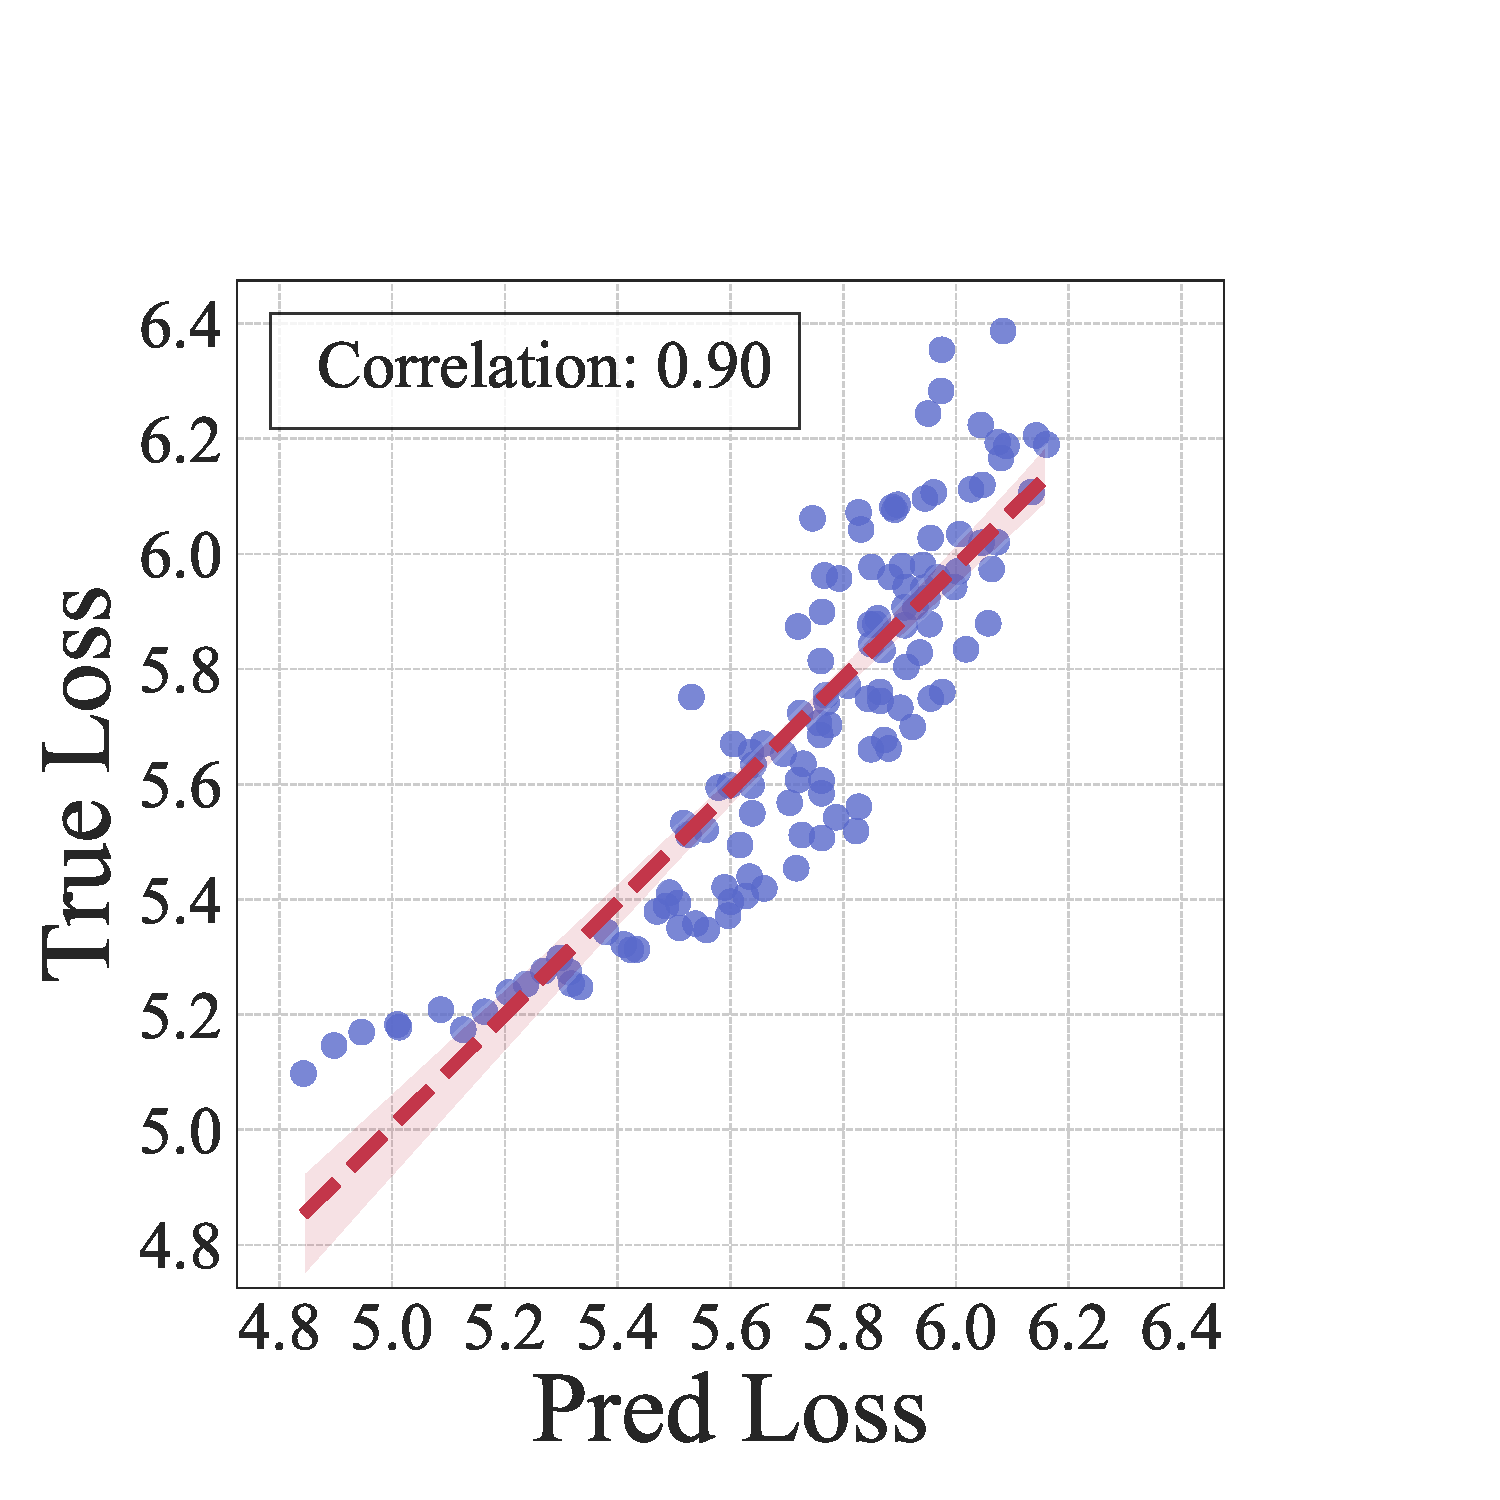
\includegraphics[width=0.45\textwidth]{figures/1M_pile_cc_Joint_linear.pdf}}
    \subfigure{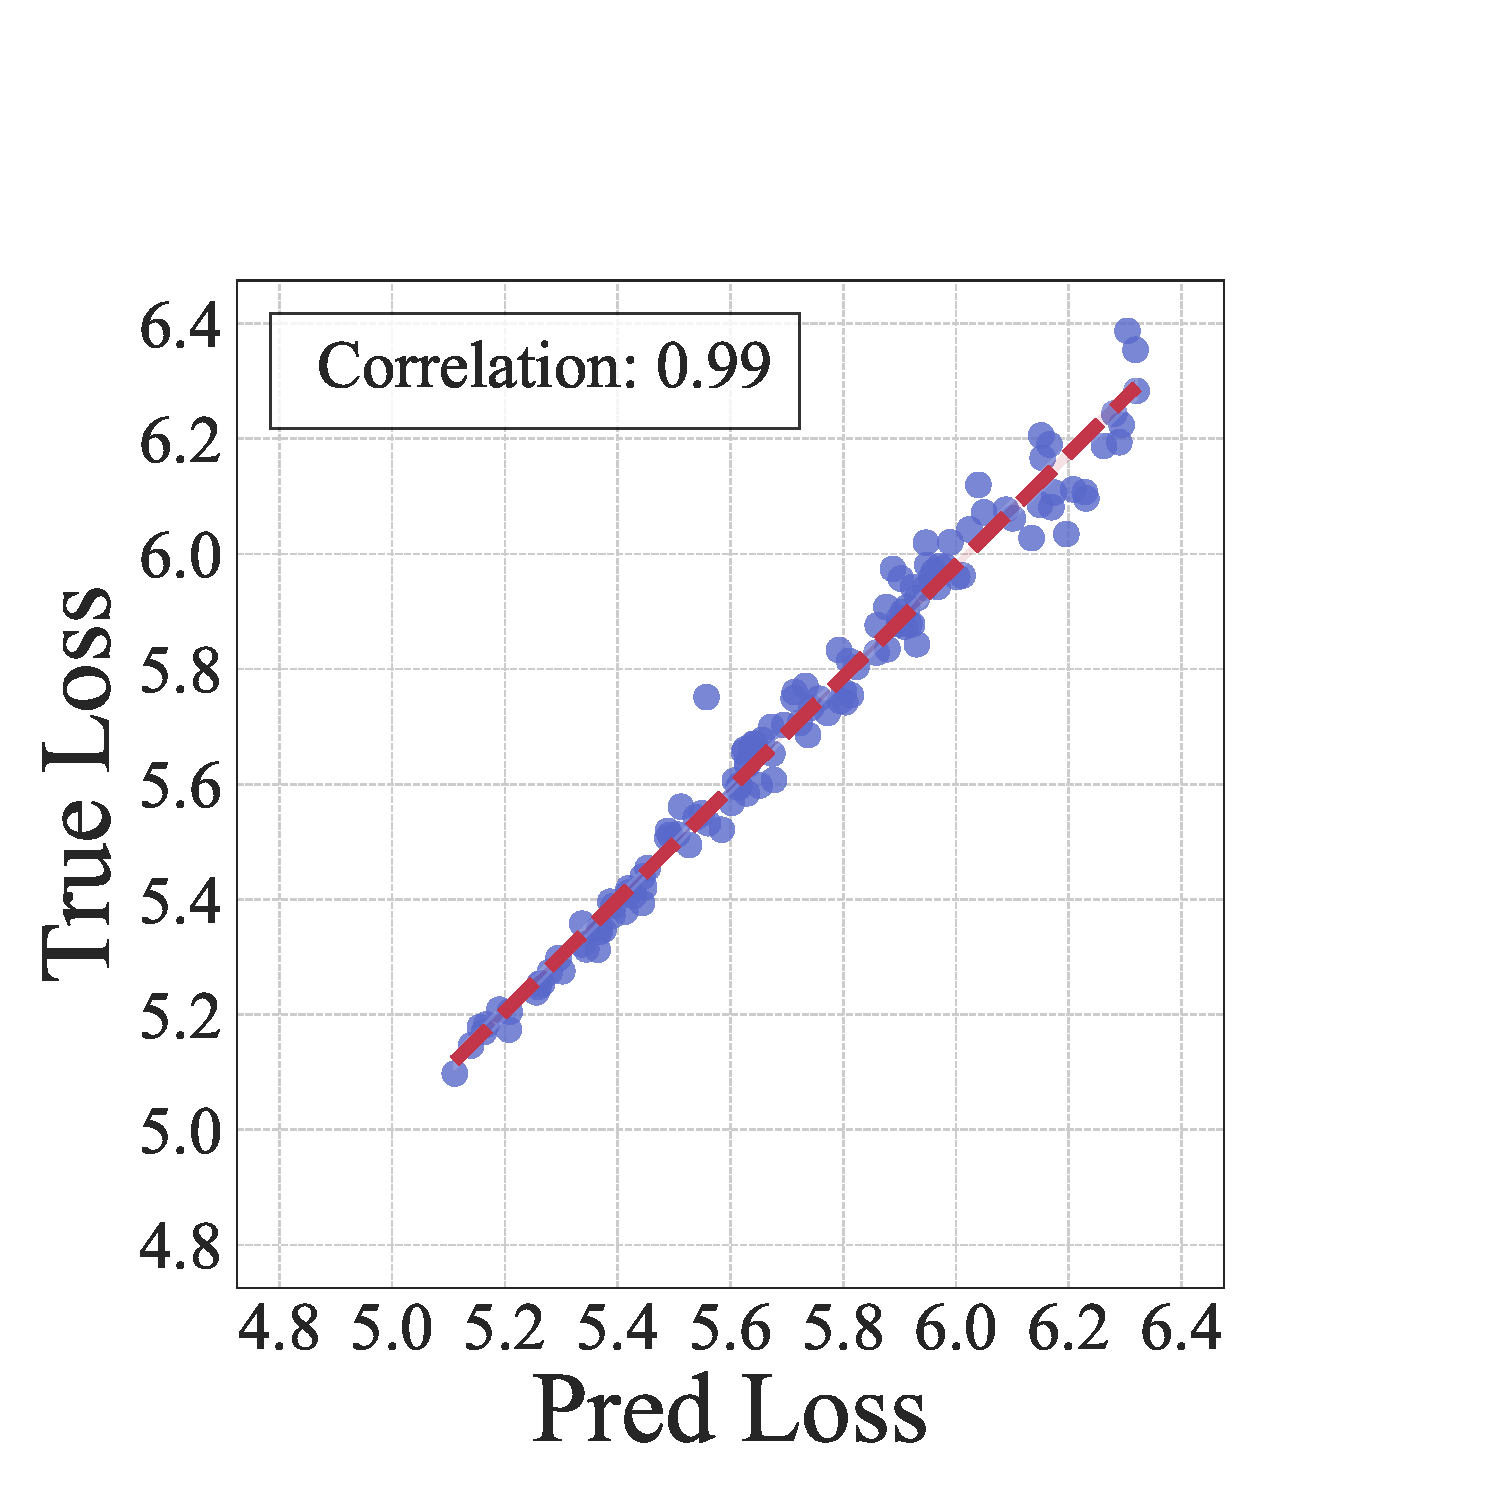
\includegraphics[width=0.45\textwidth]{figures/1M_pile_cc_Joint.pdf}}
    \caption{The visualization of loss prediction on small models (e.g., 1M parameters). \textbf{Left}: The scatter plot of predicted and true loss pairs of Linear model. \textbf{Right}: The scatter plot of predicted and true loss pairs of LightGBM model.}
    \label{fig:1M-to-128-1M-Joint}
\end{figure}


\subsection{Loss and rank prediction on small models for out-of-distribution setting}

In Section~\ref{sec:app}, we verify the effectiveness of our method in out-of-distribution scenarios where we fully exclude the Pile-CC domain from the pre-training corpus and use the remaining domains to find the optimal data mixture that minimizes Pile-CC validation loss. 
We also provide the results of regression evaluation under this setting in Figure~\ref{tab:linear_vs_lightgbm_1M_OOD}.
Similarly, LightGBM model outperforms the linear model and achieves nearly 100\% Spearman Rank Correlation $\rho$.

\begin{table}[htbp]
    \centering
    \small
    \caption{The regression model is fitted using the training artifacts of $512 \times$ 1M models trained with 1B tokens excluding the Pile-CC domain, and evaluated on \textbf{unseen data mixtures} for 1M parameter models. Pearson's r and MSE measure the loss prediction performance, while $\rho$ compares the predicted and actual ranks.}
    \label{tab:linear_vs_lightgbm_1M_OOD}
    \begin{tabular}{lccc}
        \toprule
        {Method} & \multicolumn{3}{c}{1M models with 1B tokens}\\
        \cmidrule(r){1-1} \cmidrule(lr){2-4}
        & $\rho$ ($\uparrow$) & 
        Pearson's $r$ ($\uparrow$) & MSE ($\downarrow$) \\
        \midrule
        Linear  & 83.00 & 84.18 & 0.08  \\
        LightGBM & \textbf{95.47} & \textbf{95.48} & \textbf{0.04} \\
        \bottomrule
    \end{tabular}
\end{table}

\subsection{The derived data mixtures}

Table~\ref{tab:data_mixture_all} presents the derived data mixture weights for different methods. As illustrated, \ourmethod assigns a high weight of 0.87 to the Pile-CC dataset, aligning with human intuition.


\begin{table}[t]
    \centering
    \caption{The domain weights of different methods. In our experiments, DoReMi refers to the reported best reference model with 280M parameters and its corresponding domain weights. $^\dagger$Note that the domain weights of Human and DoReMi are re-normalized from the weights reported in~\citet{xie2023doremi} to adapt them to the available domains. The DoReMi weight are derived from the best-performing configuration obtained using a 280M parameter model.}
    \label{tab:data_mixture_all}
\begin{threeparttable}
    \begin{tabular}{l|cccc}
    \toprule
        \textbf{Domain Weights} & \textbf{Human}$^\dagger$ & \textbf{DoReMi}$^\dagger$ & \textbf{Pile-CC Only} & \textbf{\ourmethod} \\
        \midrule
        ArXiv & 0.134  & 0.004  & 0.0 & 0.001 \\ 
        FreeLaw & 0.049  & 0.005  & 0.0 & 0.001 \\ 
        NIH ExPorter & 0.007  & 0.008  & 0.0 & 0.001 \\ 
        PubMed Central & 0.136  & 0.006  & 0.0 & 0.003 \\ 
        Wikipedia (en) & 0.117  & 0.086  & 0.0 & 0.016 \\ 
        DM Mathematics & 0.025  & 0.002  & 0.0 & 0.0 \\ 
        Github & 0.054  & 0.022  & 0.0 & 0.0 \\ 
        PhilPapers & 0.003  & 0.034  & 0.0 & 0.0 \\ 
        Stack Exchange & 0.118  & 0.019  & 0.0 & 0.0 \\ 
        Enron Emails & 0.004  & 0.009  & 0.0 & 0.002 \\ 
        Gutenberg (PG-19) & 0.025  & 0.009  & 0.0 & 0.002 \\ 
        Pile-CC & 0.142  & 0.743  & 1.0 & {0.87} \\ 
        Ubuntu IRC & 0.009  & 0.011  & 0.0 & {0.064} \\ 
        EuroParl & 0.005  & 0.008  & 0.0 & 0.0 \\ 
        HackerNews & 0.01  & 0.016  & 0.0 & {0.012} \\ 
        PubMed Abstracts & 0.107  & 0.014  & 0.0 & {0.024} \\ 
        USPTO Backgrounds & 0.053 & 0.004 & 0.0 & 0.002 \\
    \bottomrule
    \end{tabular}
    \end{threeparttable}
\end{table}

\subsection{The evaluation results using LightEval}\label{appendix:lighteval}


\begin{table}[tb]
    \centering
    \small
    \caption{Performance comparison of different data selection methods using LightEval following previous work~\citep{penedo2024finewebdatasetsdecantingweb}. Human refers to the weights put forth in The Pile~\citep{the_pile_corpus}, Pile-CC Only to only training on the Pile-CC component, and DoReMi to the weights from \citet{xie2023doremi}. The reported performance for each task is the average \textit{zero-shot task performance} across five different runs, and the standard deviation. We estimate the compute (measured in FLOPs) required to arrive at the training data mixture. Scores significantly outperforming the Human baseline for each task are highlighted in \textbf{bold}, with significance determined using Cohen's d. }
    \vspace{1mm}
    \label{tab:downstream_lighteval}
    \begin{tabular}{l|l|lll}
    \toprule
         \textbf{Benchmark} & \textbf{Human} & \textbf{DoReMi} & \textbf{Pile-CC Only} & \textbf{\ourmethod} \\
    \midrule
        ARC Easy~\citep{clark2018think} & 45.3\text{\,\scriptsize$\pm$\,0.4} &  {\textbf{46.6}}\text{\,\scriptsize$\pm$\,0.7} &  \textbf{47.1}\text{\,\scriptsize$\pm$\,0.6} & \textbf{47.2}\text{\,\scriptsize$\pm$\,0.9}  \\ 
        ARC Challenge~\citep{clark2018think} & 25.5\text{\,\scriptsize$\pm$\,0.8} & {25.9}\text{\,\scriptsize$\pm$\,0.8} & 25.6\text{\,\scriptsize$\pm$\,0.5} & 25.6\text{\,\scriptsize$\pm$\,0.5}  \\ 
        CommonsenseQA~\citep{talmor-etal-2019-commonsenseqa} & 31.8\text{\,\scriptsize$\pm$\,1.2} & {\textbf{34.1}}\text{\,\scriptsize$\pm$\,0.7} & \textbf{34.9}\text{\,\scriptsize$\pm$\,0.3} & \textbf{35.0}\text{\,\scriptsize$\pm$\,0.5}  \\ 
        HellaSwag~\citep{zellers2019hellaswag} & 36.5\text{\,\scriptsize$\pm$\,0.2} & \textbf{41.5}\text{\,\scriptsize$\pm$\,0.3} & \textbf{39.7}\text{\,\scriptsize$\pm$\,0.5} & \textbf{42.1}\text{\,\scriptsize$\pm$\,0.3}  \\ 
        OpenBookQA~\citep{mihaylov2018can} & {29.8}\text{\,\scriptsize$\pm$\,0.6} & \textbf{31.0}\text{\,\scriptsize$\pm$\,0.8} & \textbf{31.5}\text{\,\scriptsize$\pm$\,0.4} & \textbf{31.8}\text{\,\scriptsize$\pm$\,0.8}  \\ 
        PiQA~\citep{bisk2020piqa} &  65.4\text{\,\scriptsize$\pm$\,0.6} & \textbf{68.7}\text{\,\scriptsize$\pm$\,0.3} & \textbf{69.0}\text{\,\scriptsize$\pm$\,0.5} & \textbf{69.4}\text{\,\scriptsize$\pm$\,0.5}  \\ 
        Social IQA~\citep{sap2019socialiqa} & {41.7}\text{\,\scriptsize$\pm$\,0.3} &  42.0\text{\,\scriptsize$\pm$\,\,0.2} &  \textbf{42.7}\text{\,\scriptsize$\pm$\,0.3} &  \textbf{42.6}\text{\,\scriptsize$\pm$\,0.7}  \\ 
        WinoGrande~\citep{sakaguchi2021winogrande} & 51.1\text{\,\scriptsize$\pm$\,1.0}  & {51.2}\text{\,\scriptsize$\pm$\,0.4}  & 50.7\text{\,\scriptsize$\pm$\,1.0}  & {50.9}\text{\,\scriptsize$\pm$\,0.4}   \\ 
        MMLU~\citep{MMLU2021} & 28.6\text{\,\scriptsize$\pm$\,0.2}  & {28.9}\text{\,\scriptsize$\pm$\,0.4}  & 28.5\text{\,\scriptsize$\pm$\,0.2}  & {28.7}\text{\,\scriptsize$\pm$\,0.3}   \\ 
        \midrule
        Average Performance & 39.5\text{\,\scriptsize$\pm$\,0.3} & {41.1}\text{\,\scriptsize$\pm$\,0.3} & {41.2}\text{\,\scriptsize$\pm$\,0.3} & {41.5}\text{\,\scriptsize$\pm$\,0.2} \\
        Beat Human on & -- & 5 / 9 & 6 / 9 & 6 / 9 \\
        Estimated FLOPs & 0 & $3.7\times10^{19}$ & 0 & $3.5\times10^{18}$ \\
    \bottomrule
    \end{tabular}
\end{table}

Following the approach of FineWeb~\citep{penedo2024finewebdatasetsdecantingweb}, we employ the LightEval~\footnote{\url{https://github.com/huggingface/lighteval}} library to evaluate our models using a suite of benchmarks selected for their stability and suitability. The chosen benchmarks exhibit three key characteristics: low score variance across different data samples, monotonic score improvement during training, and above-random baseline scores for models in the 1B parameter range.
Table~\ref{tab:downstream_lighteval} presents the evaluation results. Our method, \ourmethod, consistently outperforms the Human baseline on 6 benchmarks. Moreover, \ourmethod demonstrates superior average performance compared to the DoReMi and the Pile-CC Only methods.



\clearpage
\section{URL domain correlation graph}\label{appendix:correaltion_graph}

\begin{figure}[htbp]
    \centering
    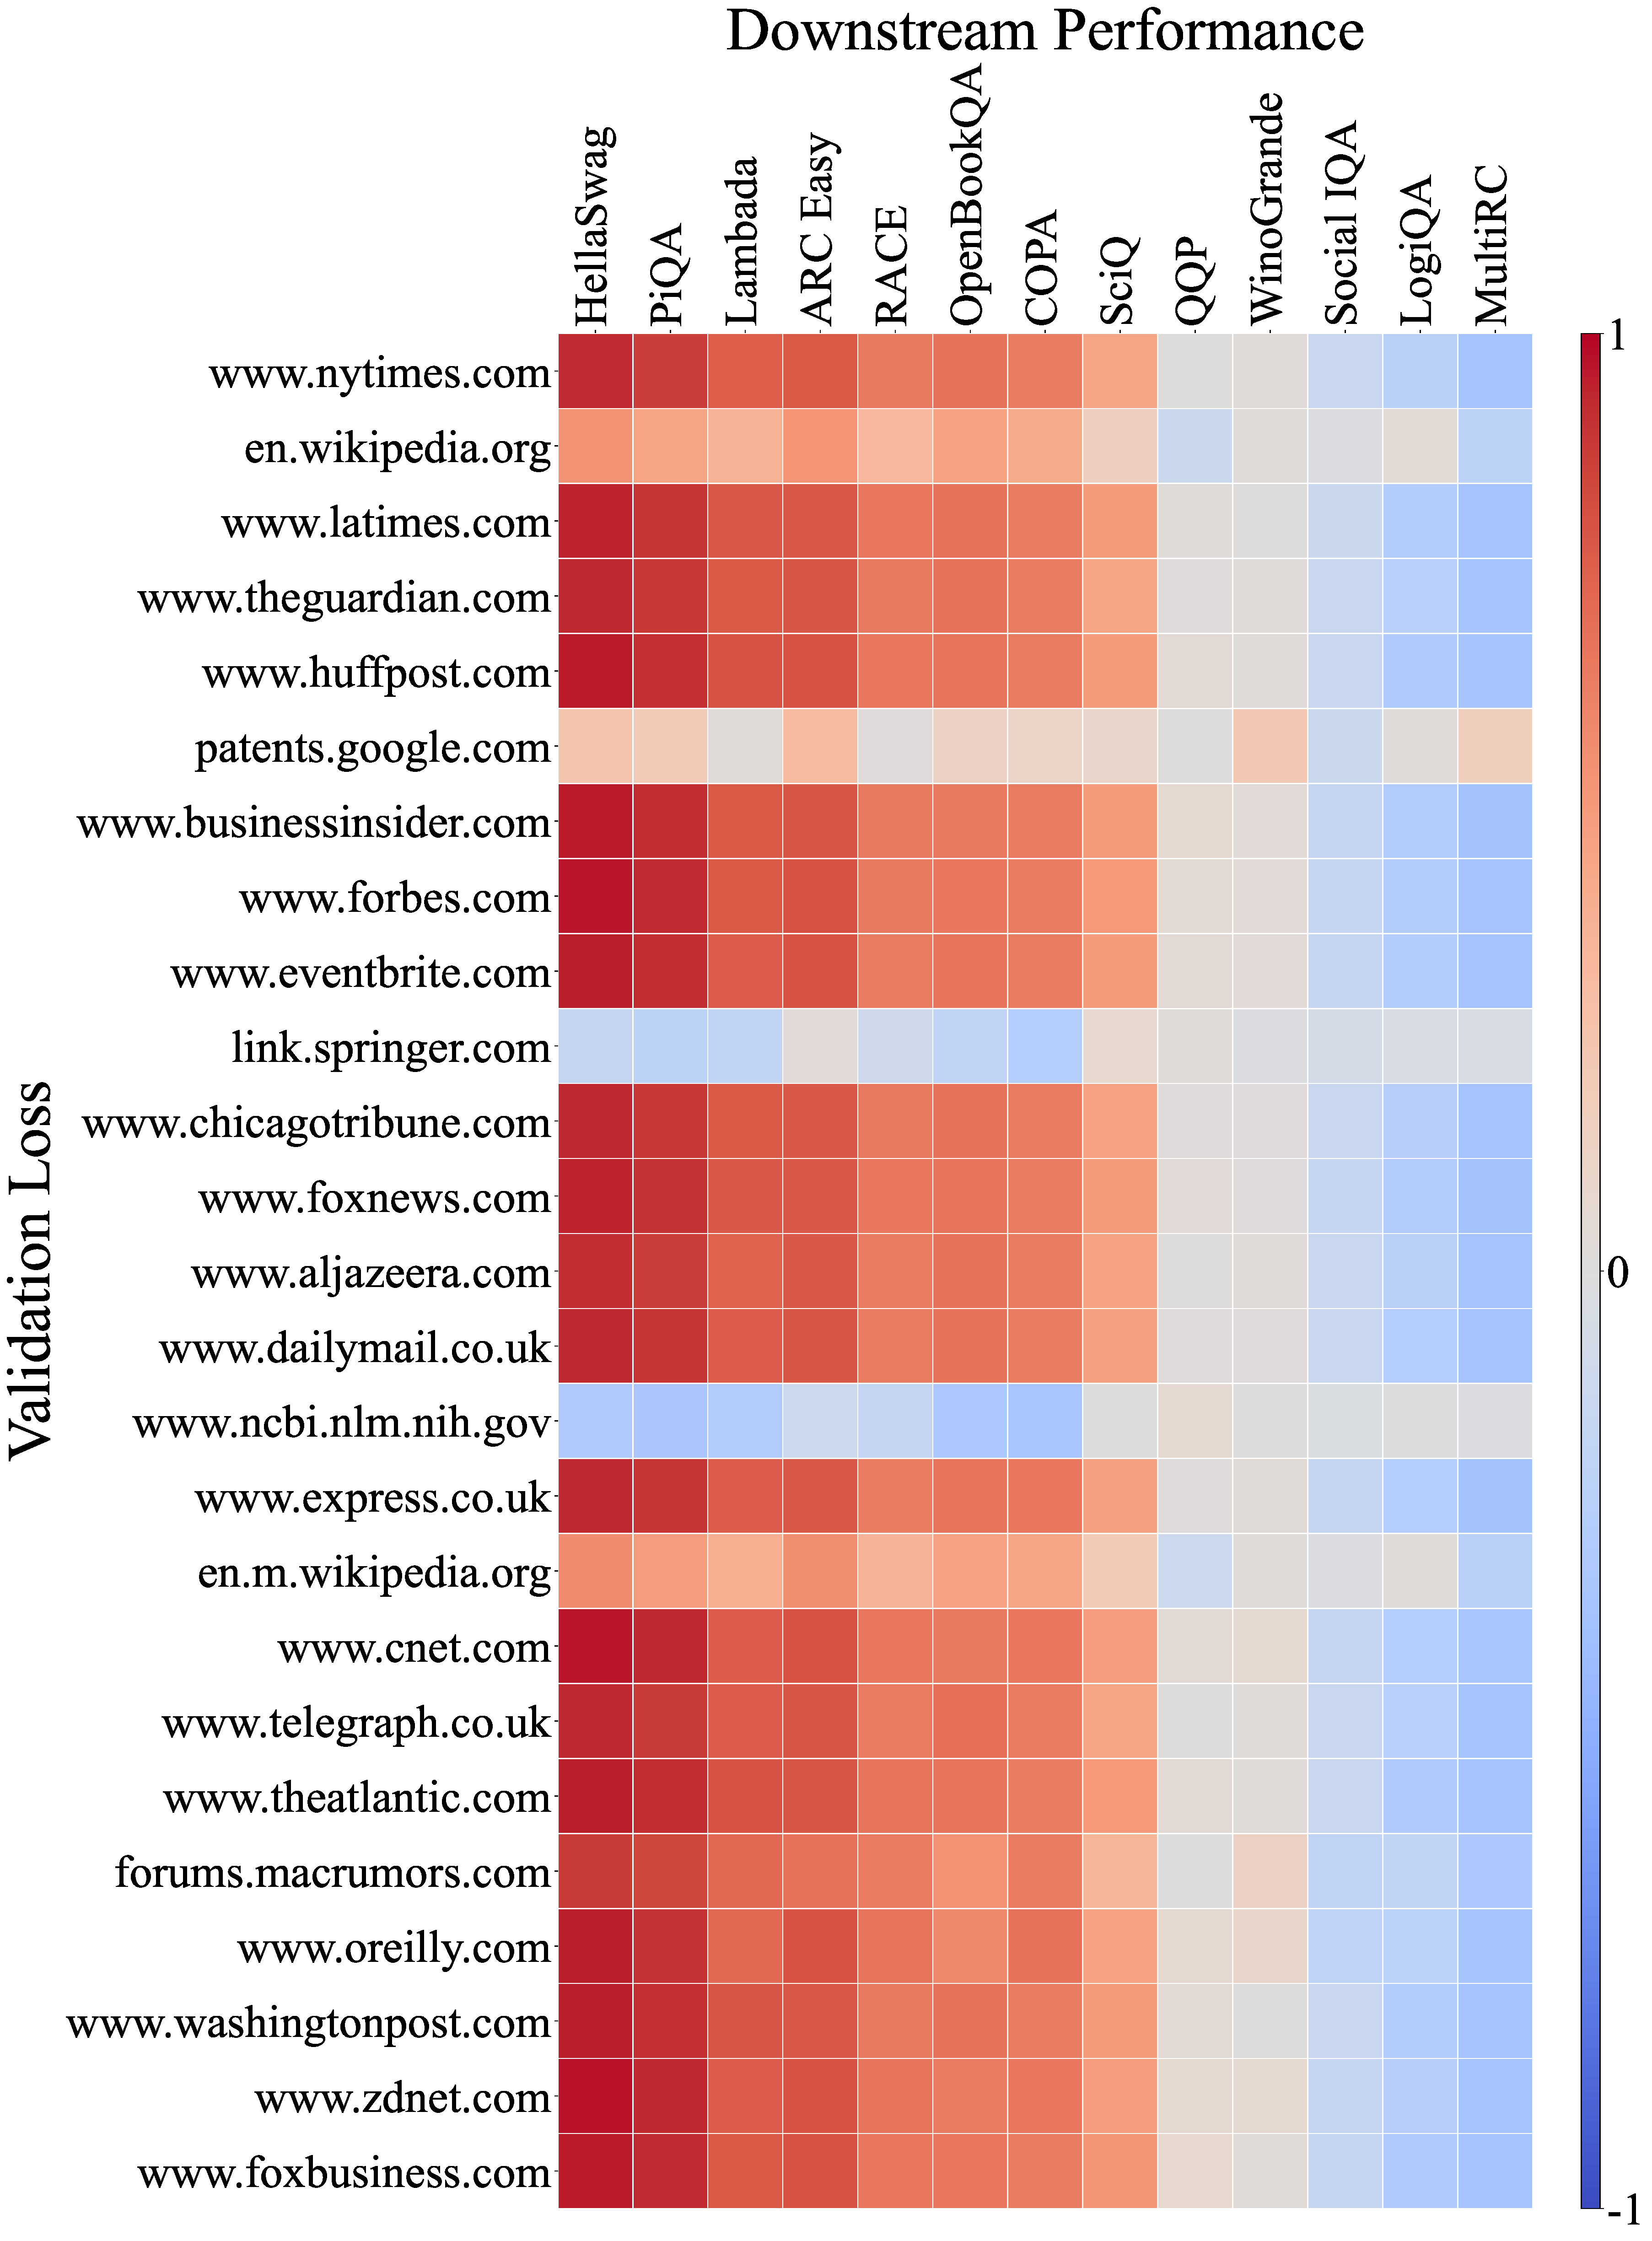
\includegraphics[height=0.9\textwidth]{figures/Domain_and_Task_c4100_full_1.pdf}
    \caption{The visualization of correlations between different URL domains within the C4 subsets and the downstream performance (Part 1).}
    \label{fig:c4100-full-1}
\end{figure}

\begin{figure}[htbp]
    \centering
    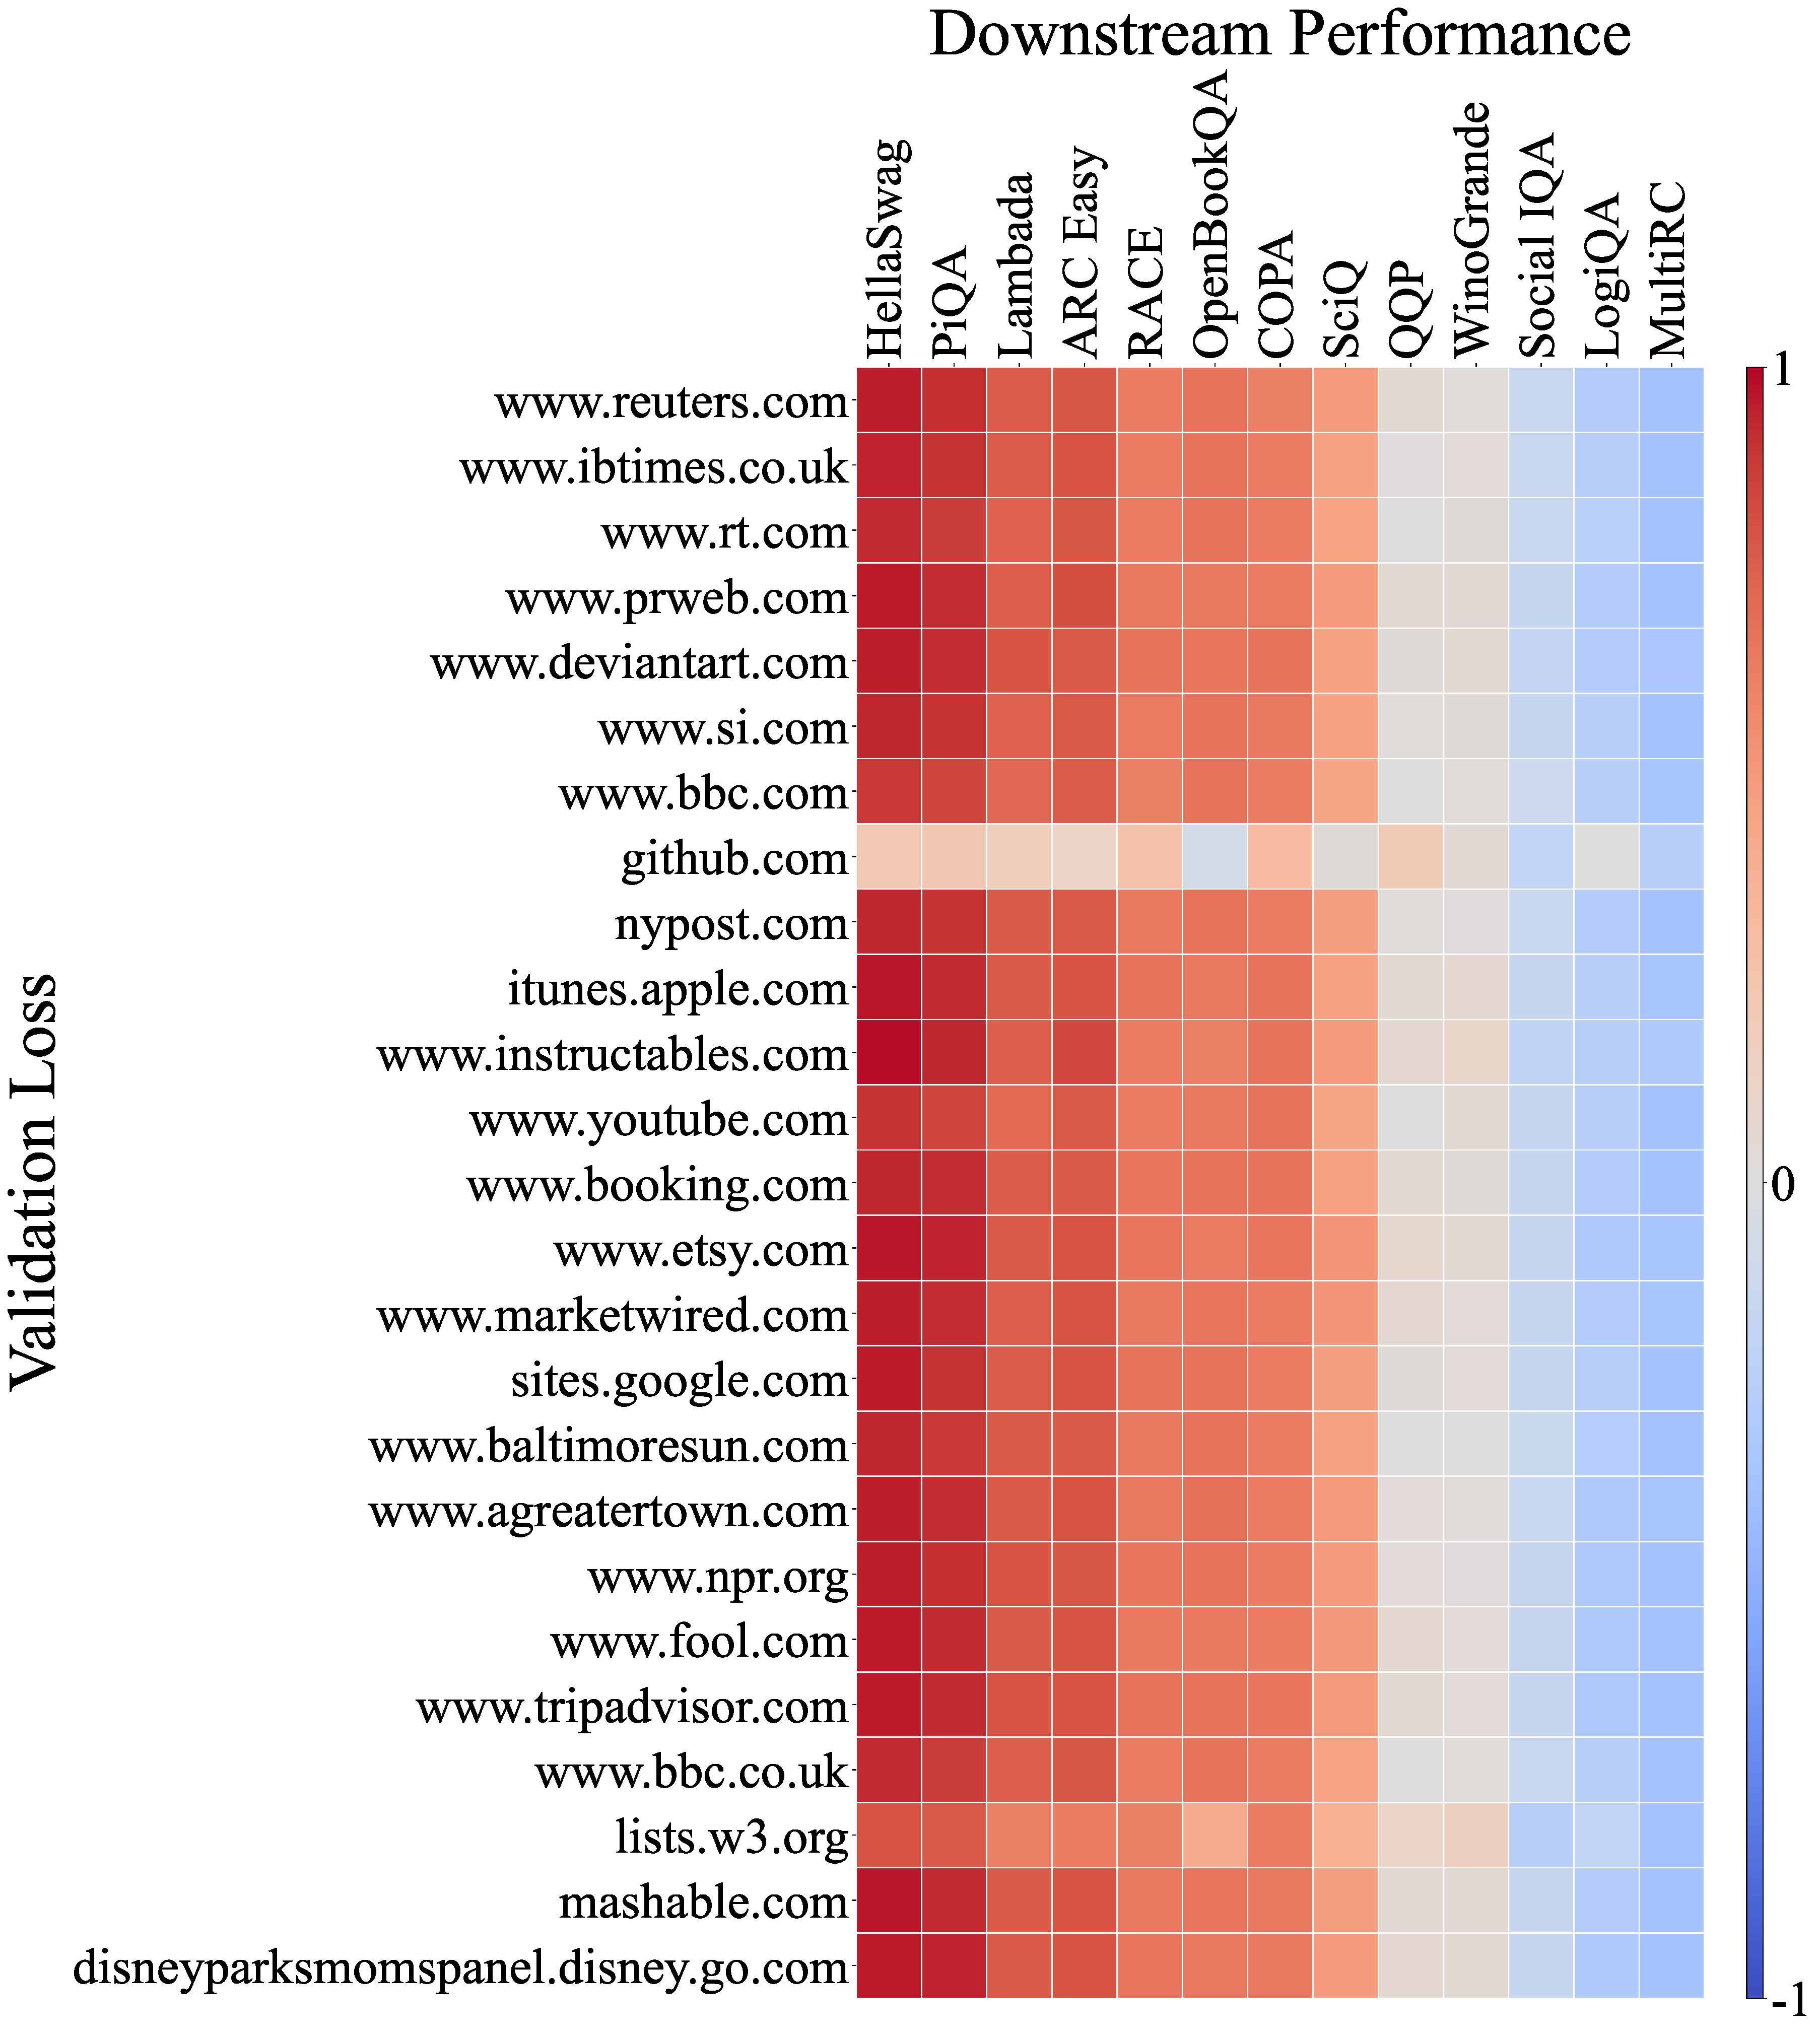
\includegraphics[height=0.9\textwidth]{figures/Domain_and_Task_c4100_full_2.pdf}
    \caption{The visualization of correlations between different URL domains within the C4 subsets and the downstream performance (Part 2).}
    \label{fig:c4100-full-2}
\end{figure}

\begin{figure}[htbp]
    \centering
    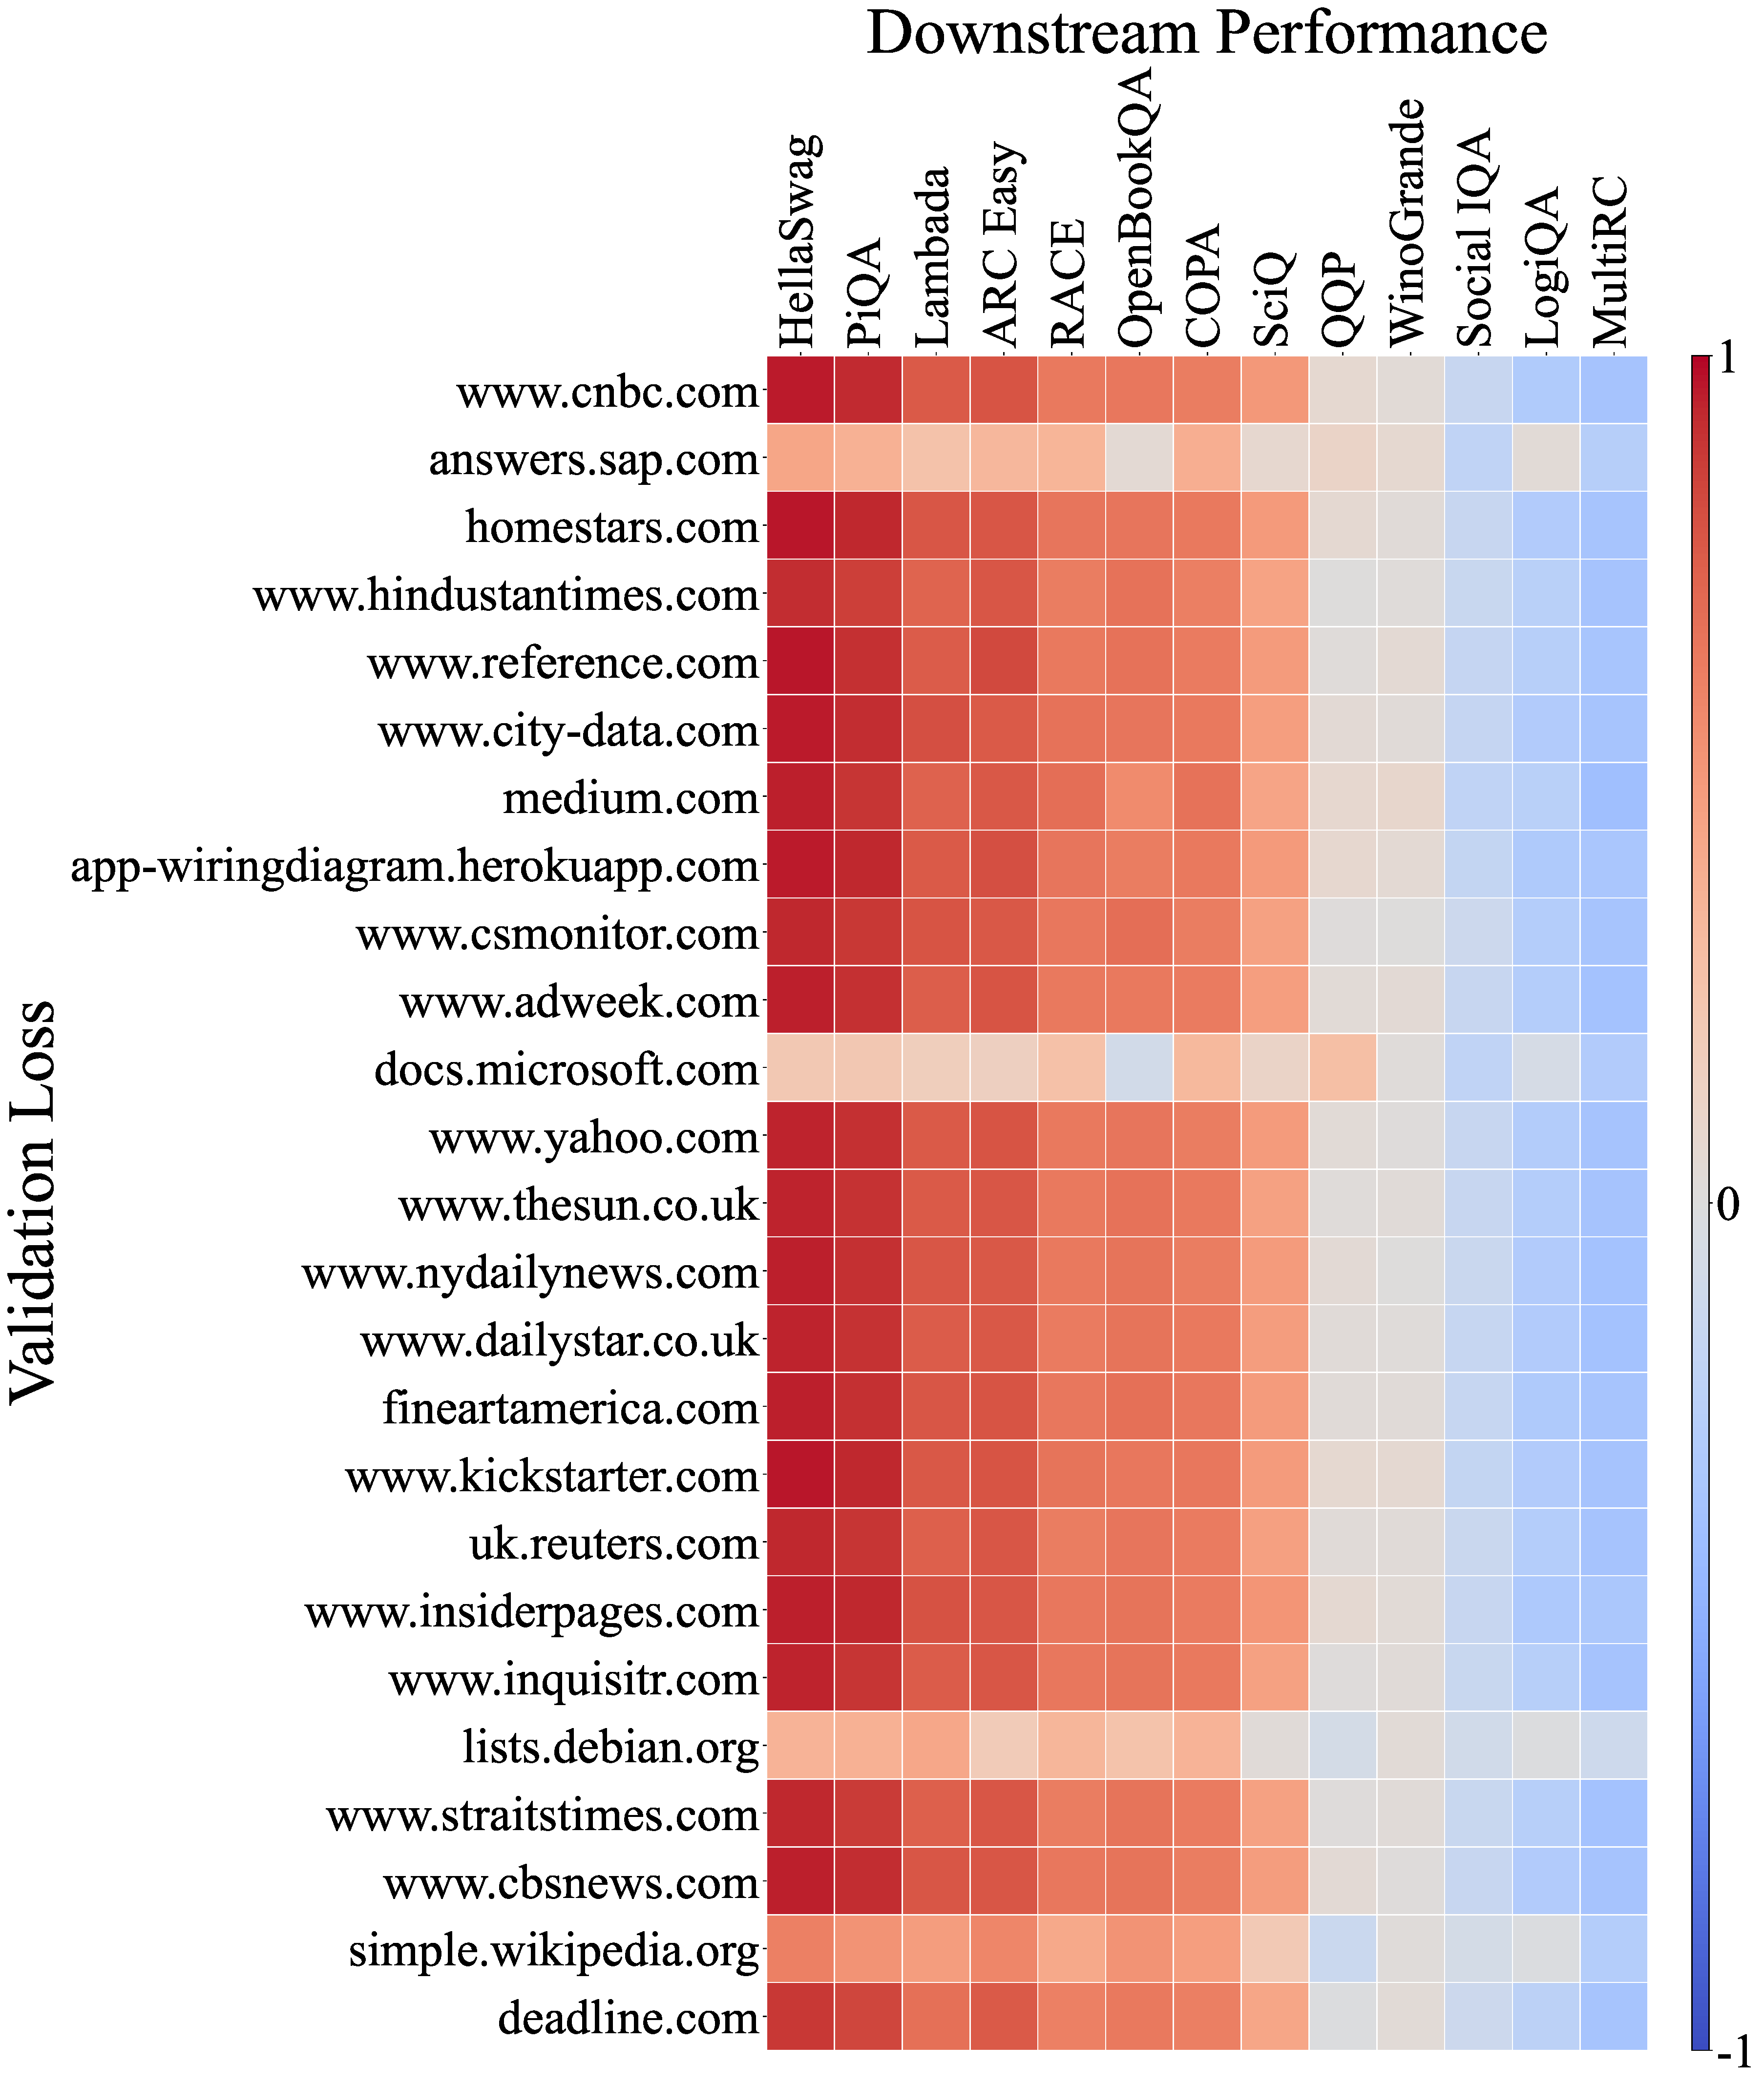
\includegraphics[height=0.9\textwidth]{figures/Domain_and_Task_c4100_full_3.pdf}
    \caption{The visualization of correlations between different URL domains within the C4 subsets and the downstream performance (Part 3).}
    \label{fig:c4100-full-3}
\end{figure}

\begin{figure}[htbp]
    \centering
    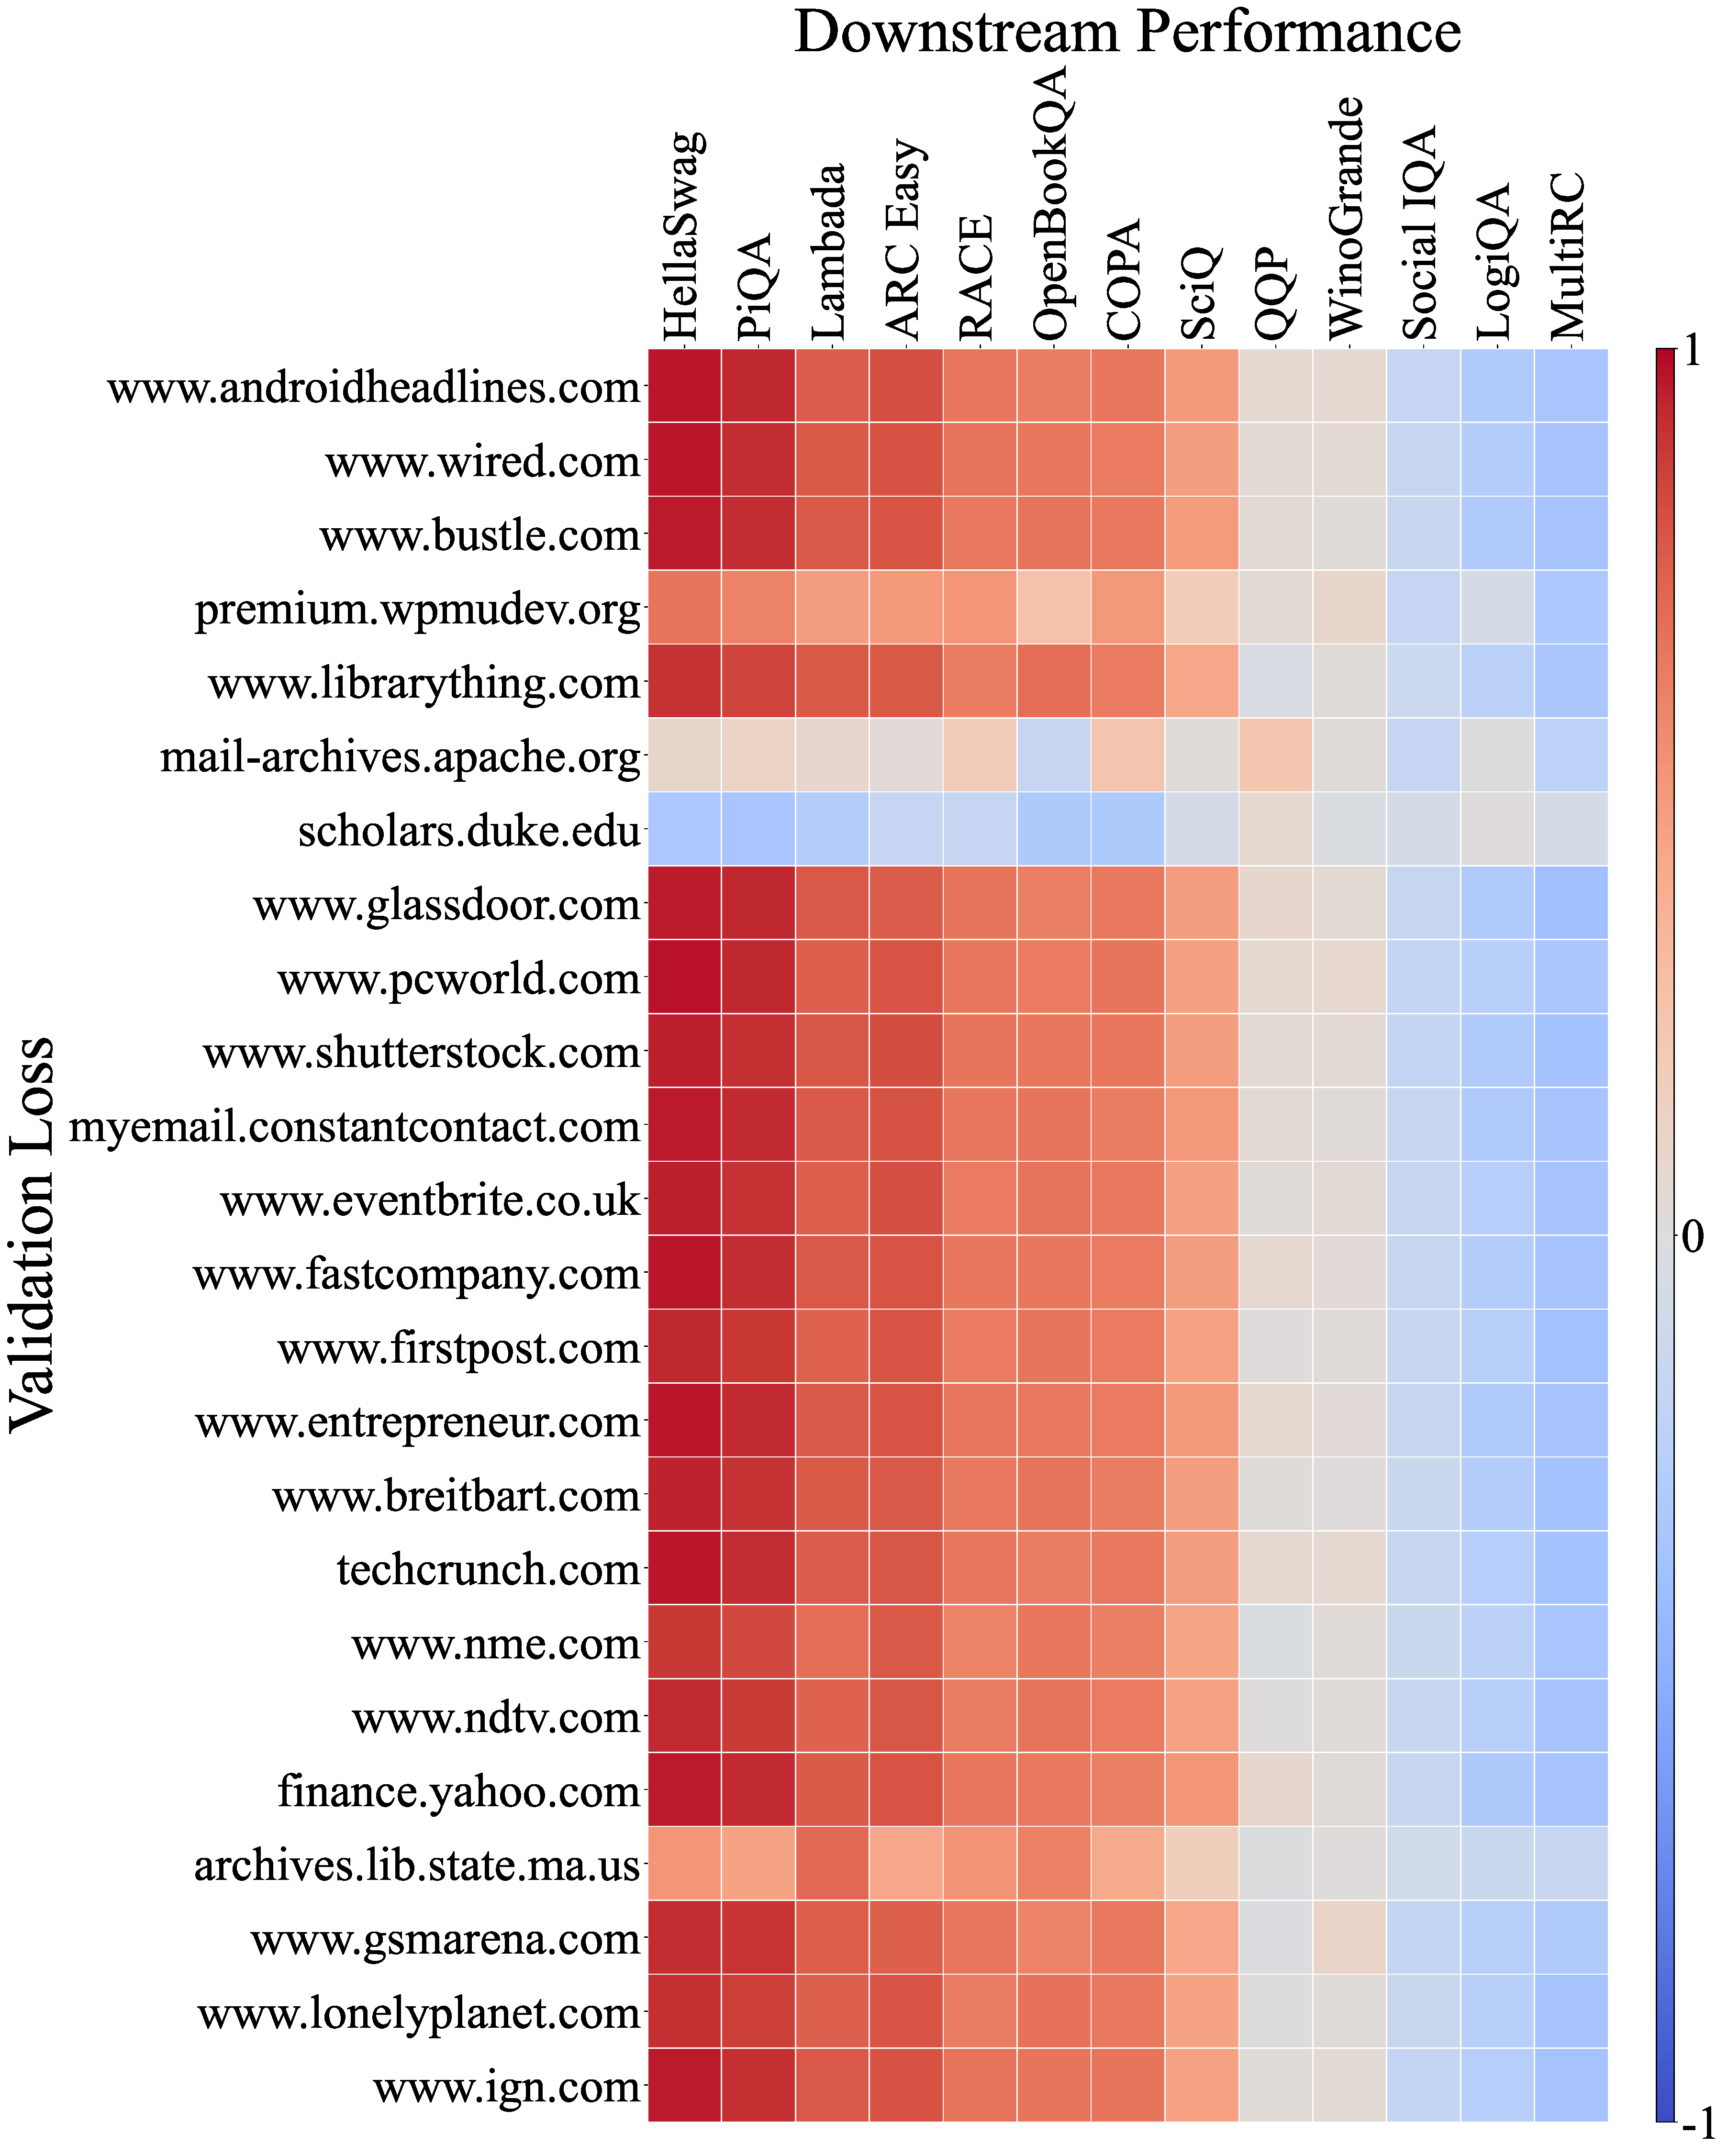
\includegraphics[height=0.9\textwidth]{figures/Domain_and_Task_c4100_full_4.pdf}
    \caption{The visualization of correlations between different URL domains within the C4 subsets and the downstream performance (Part 4).}
    \label{fig:c4100-full-4}
\end{figure}


\clearpage